\documentclass[14pt]{beamer}

\usepackage{xcolor}
\usepackage{colortbl}
\usepackage{pgf}
\usepackage{amsmath}
\usepackage{amssymb}
\usepackage{latexsym}
\usepackage{tikz}
\usepackage{pgfplots}
\usepackage{pdfpages}
\usepackage{ulem}

\newcommand{\hsc}[1]{{\footnotesize\MakeUppercase{#1}}}

%\includeonlyframes{goal}
\usepackage{rotating}

\usetikzlibrary{positioning, shapes}
\usetikzlibrary{decorations.pathmorphing}

\definecolor{shaded}{RGB}{70,60,255}
\usecolortheme[named=shaded]{structure}

\definecolor{stressed}{RGB}{150,40,40}
\setbeamercolor{alerted_text}{fg=stressed}

\setbeamertemplate{navigation symbols}{}
\setbeamersize{text margin left=3mm} 
\setbeamersize{text margin right=3mm} 

\setbeamertemplate{sidebar right}{default}{}

\makeatletter
\define@key{beamerframe}{nofills}[true]{% top
  \beamer@frametopskip=0pt\relax%
  \beamer@framebottomskip=0pt\relax%
  \beamer@frametopskipautobreak=\beamer@frametopskip\relax%
  \beamer@framebottomskipautobreak=\beamer@framebottomskip\relax%
  \def\beamer@initfirstlineunskip{%
    \def\beamer@firstlineitemizeunskip{%
      \vskip-\partopsep\vskip-\topsep\vskip-\parskip%
      \global\let\beamer@firstlineitemizeunskip=\relax}%
    \everypar{\global\let\beamer@firstlineitemizeunskip=\relax}}
}
\makeatother

\newcommand{\defnword}[1]{\textbf{#1}}

\usepackage{amsthm}
\newtheorem*{conjecture}{Conjecture}

\newtheorem{observation}[theorem]{Observation}
%\newtheorem{definition}[theorem]{Definition}
\newtheorem{remark}[theorem]{Remark}
\newtheorem{claim}[theorem]{Claim}
\newtheorem{proposition}[theorem]{Proposition}
\newtheorem{question}[theorem]{Question}

\newcommand{\Z}{\mathbb{Z}}
\newcommand{\Q}{\mathbb{Q}}
\newcommand{\R}{\mathbb{R}}
\newcommand{\OO}{\mathbb{O}}
\newcommand{\HH}{\mathbb{H}}
\newcommand{\RP}{\mathbb{R}P}
\newcommand{\CP}{\mathbb{C}P}
\newcommand{\HP}{\mathbb{H}P}
\newcommand{\OP}{\mathbb{O}P}
\DeclareMathOperator{\Spin}{Spin}
\DeclareMathOperator{\Homeo}{Homeo}
\DeclareMathOperator{\SO}{SO}
\DeclareMathOperator{\fiber}{fiber}
\DeclareMathOperator{\proj}{proj}

\newcommand{\LL}{\mathbb{L}}
\newcommand{\setbackgroundblack}{%
\usebackgroundtemplate{
\begin{pgfpicture}{0in}{0in}{\paperwidth}{\paperheight}
\color{black}
\pgfrect[fill]{\pgfxy(0,0)}{\pgfpoint{\paperwidth}{\paperheight}}
\end{pgfpicture}
}
}

\newcommand{\setbackgroundgreen}{%
\usebackgroundtemplate{
\begin{pgfpicture}{0in}{0in}{\paperwidth}{\paperheight}
\color{red!50!black}
\pgfrect[fill]{\pgfxy(0,0)}{\pgfpoint{\paperwidth}{\paperheight}}
\end{pgfpicture}
}
}

\newcommand{\sectionslide}[1]{%
\setbackgroundblack
\begin{frame}[nofills]
\Huge
\vfill
\scaletowidth{\textwidth}{\textcolor{white}{\textbf{#1}}}
\vfill
\end{frame}
\clearbackgroundpicture
}

\newcommand{\encouragement}[1]{%
\setbackgroundgreen
\begin{frame}[nofills]
\Huge
\vfill
\scaletowidth{\textwidth}{\textcolor{white}{#1}}
\vfill
\end{frame}
\clearbackgroundpicture
}

\definecolor{FootColor}{rgb}{0.322,0.322,0.322}%
\definecolor{FootBackgroundColor}{rgb}{1,1,1}%

\setbeamercolor{bottomcolor}{fg=black,bg=gray!15!white}

%%%%%%%%%%%%%%%%%%%%%%%%%%%%%%%%%%%%%%%%%%%%%%%%%%%%%%%%%%%%%%%%
% stack two things so that they have the same size
\newlength{\firstline}
\newlength{\secondline}
\newcommand{\stacksame}[2]{%
\setlength{\firstline}{\widthof{#1}}%
\setlength{\secondline}{\widthof{#2}}%
\pgfmathsetmacro{\myratio}{\firstline/\secondline}%
\shortstack{#1\\\scalebox{\myratio}{#2}}}

\newlength{\myscalewidth}
\newcommand{\scaletowidth}[2]{%
\setlength{\myscalewidth}{\widthof{#2}}%
\pgfmathsetmacro{\myscaleratio}{#1/\myscalewidth}%
\scalebox{\myscaleratio}{#2}}

%%%%%%%%%%%%%%%%%%%%%%%%%%%%%%%%%%%%%%%%%%%%%%%%%%%%%%%%%%%%%%%%
% I like words in front of faded images

\newcommand{\setbackgroundpicturewhite}[1]{%
\definecolor{FootColor}{rgb}{0.322,0.322,0.322}%
\definecolor{FootBackgroundColor}{rgb}{1,1,1}%
\setbeamercolor{bottomcolor}{fg=black,bg=gray!15!white}%
\usebackgroundtemplate{%
\begin{tikzpicture}[overlay,remember picture]%
\draw[fill=white] (current page.north west) rectangle (current page.south east);%
\node[fill=white,minimum width=\paperwidth,minimum height=\paperheight,yshift=1.5mm] [anchor=north west] (mynode) {\hspace{-1.5mm}\includegraphics[width=\paperwidth]{#1}};%
\end{tikzpicture}%
}}


\newcommand{\settallbackgroundpicturewhite}[1]{%
\definecolor{FootColor}{rgb}{0.322,0.322,0.322}%
\definecolor{FootBackgroundColor}{rgb}{1,1,1}%
\setbeamercolor{bottomcolor}{fg=black,bg=gray!15!white}%
\usebackgroundtemplate{%
\begin{tikzpicture}[overlay,remember picture]%
\draw[fill=white] (current page.north west) rectangle (current page.south east);%
\node[minimum width=\paperwidth,minimum height=\paperheight,yshift=1.5mm] [anchor=north west] (mynode) {\hspace{-1.5mm}\includegraphics[height=\paperheight]{#1}};%
\end{tikzpicture}%
}}


\newcommand{\settallbackgroundpictureblack}[1]{%
\definecolor{FootColor}{rgb}{0.678,0.678,0.678}%
\definecolor{FootBackgroundColor}{rgb}{0,0,0}%
\setbeamercolor{bottomcolor}{fg=black,bg=gray!15!white}%
\usebackgroundtemplate{%
\begin{tikzpicture}[overlay,remember picture]%
\draw[fill=black] (current page.north west) rectangle (current page.south east);%
\node[minimum width=\paperwidth,minimum height=\paperheight,yshift=1.5mm] [anchor=north west] (mynode) {\hspace{-1.5mm}\includegraphics[height=\paperheight]{#1}};%
\end{tikzpicture}%
}}


\newcommand{\setbackgroundpictureblack}[1]{%
\definecolor{FootColor}{rgb}{0.678,0.678,0.678}%
\definecolor{FootBackgroundColor}{rgb}{0,0,0}%
\setbeamercolor{bottomcolor}{fg=white,bg=gray!15!black}%
\usebackgroundtemplate{%
\begin{tikzpicture}[overlay,remember picture]%
\draw[fill=black] (current page.north west) rectangle (current page.south east);%
\node[minimum width=\paperwidth,minimum height=\paperheight,yshift=1.5mm] [anchor=north west] (mynode) {\hspace{-1.5mm}\includegraphics[width=\paperwidth]{#1}};%
\end{tikzpicture}%
}}


\newcommand{\setdarkbackgroundpictureblack}[1]{%
\definecolor{FootColor}{rgb}{0.678,0.678,0.678}%
\definecolor{FootBackgroundColor}{rgb}{0,0,0}%
\setbeamercolor{bottomcolor}{fg=white,bg=gray!15!black}
\usebackgroundtemplate{%
\begin{tikzpicture}[overlay,remember picture]%
\draw[fill=black] (current page.north west) rectangle (current page.south east);%
\node[minimum width=\paperwidth,minimum height=\paperheight,yshift=1.5mm] [anchor=north west] (mynode) {\hspace{-1.5mm}\includegraphics[width=\paperwidth]{#1}};%
\draw[fill=black,opacity=0.75] (current page.north west) rectangle (current page.south east);%
\end{tikzpicture}%
}}%


\newcommand{\setdarkbackgroundpicturewhite}[1]{%
\definecolor{FootColor}{rgb}{0.322,0.322,0.322}%
\definecolor{FootBackgroundColor}{rgb}{1,1,1}%
\setbeamercolor{bottomcolor}{fg=black,bg=gray!15!white}
\usebackgroundtemplate{%
\begin{tikzpicture}[overlay,remember picture]%
\draw[fill=white] (current page.north west) rectangle (current page.south east);%
\node[minimum width=\paperwidth,minimum height=\paperheight,yshift=1.5mm] [anchor=north west] (mynode) {\hspace{-1.5mm}\includegraphics[width=\paperwidth]{#1}};%
\draw[fill=white,opacity=0.75] (current page.north west) rectangle (current page.south east);%
\end{tikzpicture}%
}}%

\newcommand{\settalldarkbackgroundpicturewhite}[1]{%
\definecolor{FootColor}{rgb}{0.322,0.322,0.322}%
\definecolor{FootBackgroundColor}{rgb}{1,1,1}%
\setbeamercolor{bottomcolor}{fg=black,bg=gray!15!white}
\usebackgroundtemplate{%
\begin{tikzpicture}[overlay,remember picture]%
\draw[fill=white] (current page.north west) rectangle (current page.south east);%
\node[minimum width=\paperwidth,minimum height=\paperheight,yshift=1.5mm] [anchor=north west] (mynode) {\hspace{-1.5mm}\includegraphics[height=\paperheight]{#1}};%
\draw[fill=white,opacity=0.75] (current page.north west) rectangle (current page.south east);%
\end{tikzpicture}%
}}%


\newcommand{\settalldarkbackgroundpictureblack}[1]{%
\definecolor{FootColor}{rgb}{0.678,0.678,0.678}%
\definecolor{FootBackgroundColor}{rgb}{0,0,0}%
\setbeamercolor{bottomcolor}{fg=black,bg=gray!15!white}
\usebackgroundtemplate{%
\begin{tikzpicture}[overlay,remember picture]%
\draw[fill=black] (current page.north west) rectangle (current page.south east);%
\node[minimum width=\paperwidth,minimum height=\paperheight,yshift=1.5mm] [anchor=north west] (mynode) {\hspace{-1.5mm}\includegraphics[height=\paperheight]{#1}};%
\draw[fill=black,opacity=0.75] (current page.north west) rectangle (current page.south east);%
\end{tikzpicture}%
}}%

\newcommand{\clearbackgroundpicture}{\usebackgroundtemplate{}%
\definecolor{FootColor}{rgb}{0.322,0.322,0.322}%
\definecolor{FootBackgroundColor}{rgb}{1,1,1}%
\setbeamercolor{bottomcolor}{fg=black,bg=gray!15!white}
}

\definecolor{osugray}{HTML}{5e6061}
\definecolor{ccgray}{HTML}{a7b1a6}

\newcommand{\whitebackground}{\setbeamercolor{background canvas}{bg=white,fg=black}\usebeamercolor[fg]{background canvas}}
\newcommand{\blackbackground}{\setbeamercolor{background canvas}{bg=black,fg=white}\usebeamercolor[fg]{background canvas}}

\begin{document}
\whitebackground

%%%%%%%%%%%%%%%%%%%%%%%%%%%%%%%%%%%%%%%%%%%%%%%%%%%%%%%%%%%%%%%%
\clearbackgroundpicture
\begin{frame}[nofills]
  \vspace{5ex}

  \large
  \scaletowidth{\textwidth}{\textbf{Switching from a Commercial Textbook to a}} \\
  \scaletowidth{\textwidth}{\textbf{Ximera OER Textbook}}

  \vfill
  
  \color{osugray}

  \begin{columns}
    \begin{column}{0.45\textwidth}
      \vfill
      \scriptsize
      \vspace{-6ex}
      \scaletowidth{\textwidth}{Imaginarium}\\[0ex]
      \scaletowidth{\textwidth}{2018 Innovate}\\[3ex]
      \scaletowidth{\textwidth}{Ohio State University} % December 9, 2017}

    \end{column}
    \hfill
    \begin{column}{0.5\textwidth}
      \vfill
      \vspace{2.5ex}
      \normalsize
      \textsf{\textbf{Jim Fowler \textcolor{osugray}{and} Bart Snapp}} \\
      \textsf{The Ohio State University} \\
      \textsf{Department of Mathematics} \\
      \vspace{0.6in}
\end{column}
\end{columns}
  
\end{frame}

\begin{frame}
  \large
  
  I am very thankful to the organizers \\
  \quad for the chance to share our project.
  %our project at Ohio State
  
  \vfill
  
  This is a joint project \\
  supported by NSF DUE--1245433, \\
  \quad the Shuttleworth Foundation, and \\
  \quad the Affordable Learning eXchange (ALX) \\
  \quad\quad at Ohio State.

  \vfill
  
\end{frame}


\begin{frame}
  \frametitle{Learning outcomes for today}
  \large
  
  \begin{itemize}
  \item Open-source isn't cheaper; it's better.
  \item Technology is empowering \\
    \quad when easy things are easy, \\
    \quad\quad and hard things aren't impossible.
  \item Research results hint at the benefits \\
    \quad of an open-source textbook.
  \end{itemize}
\end{frame}

\clearbackgroundpicture
\encouragement{Better, not cheaper.}
\clearbackgroundpicture

\begin{frame}
  \frametitle{Philosophy of the Problem}
  \large

  Among top eighty \\
  \quad Ph.D. granting math departments, \\
  \quad\quad \textbf{67\%} use an online homework system, \\
  \quad and most are commercial. \textcolor{gray}{(AMS 2009)}

  \vfill

  To ask our students to pay Pearson \\
  \quad to receive feedback on homework \\
  \quad\quad is to outsource our core mission. \\
  %\quad The most engaged students will want \\
  %\quad\quad to dig into the guts of the assessment platform.

\end{frame}

\begin{frame}
  \large

  The choice is not zero versus non-zero price. \\
  The choice is between open versus closed. 

  \vfill
  \begin{tabular}{l@{ }l@{ }l}
    What does & a closed & textbook say about learning?\\
    &an open& textbook 
  \end{tabular}

  \vfill
  
  If a \$300 book guaranteed student success, \\
  \quad we'd all just buy that---failing is costlier!
  
\end{frame}

\begin{frame}
  \frametitle{Open is better, not cheaper.}
  \large
  
  We can't beat the economies of scale \\
  \quad that publishers provide.

  \vfill
  
  Our advantage rather lies in our mastery of \\
  \quad pedagogical content knowledge.

  \vfill
  
  Why is Wikipedia better than \textit{Britannica}? \\
  \textcolor{gray}{Timely.  Expert.  Mobile.  Editable.  Bookmarkable.  Plain text.  Licensed for reuse.  Links to primary sources.  Semantic markup.  Discussions\ldots} \\ And the platform itself is open.

\end{frame}

\clearbackgroundpicture
\encouragement{What's easy?  What's hard?}
\clearbackgroundpicture

\begin{frame}
  \frametitle{Promote a particular pedagogy}
  \Large
  
  I want a platform that makes it easy to \\
  \quad present learners with some content \\
  \quad\quad (either through text or video) \\
  and helps check their understanding, \\
  \quad with hints and feedback that \\
  \quad\quad don't just tell the answer. \\

\end{frame}

\begin{frame}
  \frametitle{A Solution}
  \large

  \textbf{Ximera} converts \LaTeX\ source \\
  \quad into both paper and interactive webpages, \\
  storing student outcomes in the LMS gradebook, \\
  \quad and all the while capturing an event stream  \\
  \quad\quad that can be mined for insights about learning.

  \vfill
  
  Page state is synchronized in real-time, \\
  \quad so instructors can watch students working.

\end{frame}

\begin{frame}
  \frametitle{\TeX\ as input for computer algebra}
  \large

  The input \texttt{\$\textbackslash answer\{\textbackslash cos\^{}2 x\}\$} \\
  \quad will create an answer blank, \\
  \quad\quad the correct answer to which is $\cos^2 x$.

  \vfill
  
  \texttt{\textbackslash answer}s can be placed in surprising places, e.g., \\
  \quad\(\mbox{\texttt{\$\textbackslash sqrt\{\textbackslash frac\{1\}\{\textbackslash answer\{4\}\}\}}} \) \\
  \quad\quad\( = \mbox{\texttt{\textbackslash frac\{1\}\{2\}\$}} \)

  \vfill

  MathJax converts \texttt{\textbackslash answer}s into appropriately
  sized textfields.

  \vfill
  
\end{frame}

%%%%%%%%%%%%%%%%%%%%%%%%%%%%%%%%%%%%%%%%%%%%%%%%%%%%%%%%%%%%%%%%
\setbackgroundpicturewhite{mooculus-textbook-printed-page.pdf}
\begin{frame}[nofills]
\end{frame}

\setbackgroundpictureblack{mooculus-textbook-web-page.png}
\begin{frame}
\end{frame}


%%%%%%%%%%%%%%%%%%%%%%%%%%%%%%%%%%%%%%%%%%%%%%%%%%%%%%%%%%%%%%%%
\setbackgroundpictureblack{ximera-math-answer.png}
\begin{frame}
\end{frame}

\clearbackgroundpicture
\begin{frame}
  \large
  \frametitle{Dogfooding}

  %Ximera is the open platform.

  %Content from GitHub is automatically served on the web.

  Ohio State's math department \\
  \quad started with an open source calculus text \\
  \quad\quad written in the 1990s \\
  \quad and has edited it \\
  \quad\quad collaboratively via GitHub.

\end{frame}

\settallbackgroundpicturewhite{covers/frontCover1.pdf}
\begin{frame}
\end{frame}
\settallbackgroundpicturewhite{covers/frontCover2.pdf}
\begin{frame}
\end{frame}
\settallbackgroundpicturewhite{covers/frontCover3.pdf}
\begin{frame}
\end{frame}
\settallbackgroundpicturewhite{covers/frontCoverE.pdf}
\begin{frame}
\end{frame}
\clearbackgroundpicture

\clearbackgroundpicture
\encouragement{Research results}
\clearbackgroundpicture

\begin{frame}
  \begin{center}
    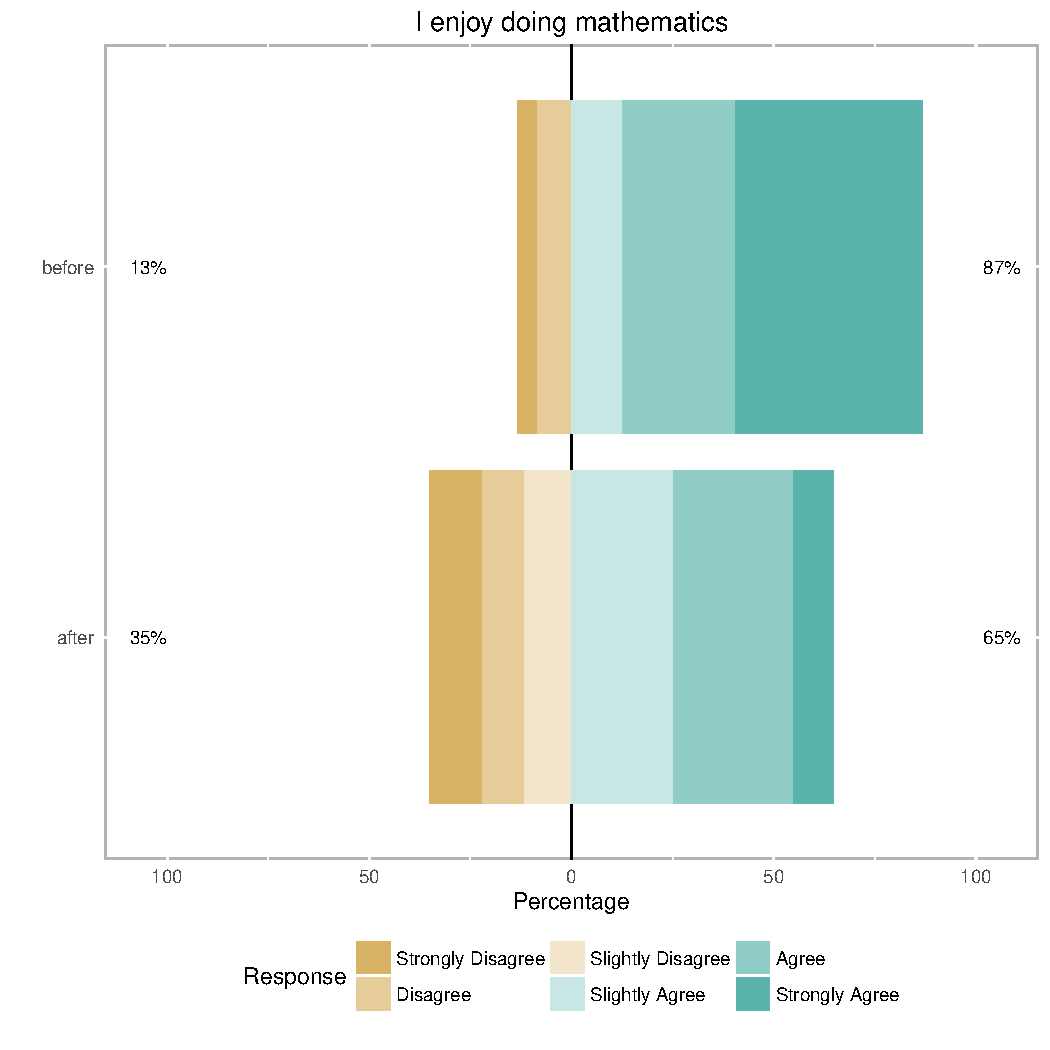
\includegraphics[height=\textheight]{graphs/enjoyment.pdf}
  \end{center}
\end{frame}

\begin{frame}
  \begin{center}
    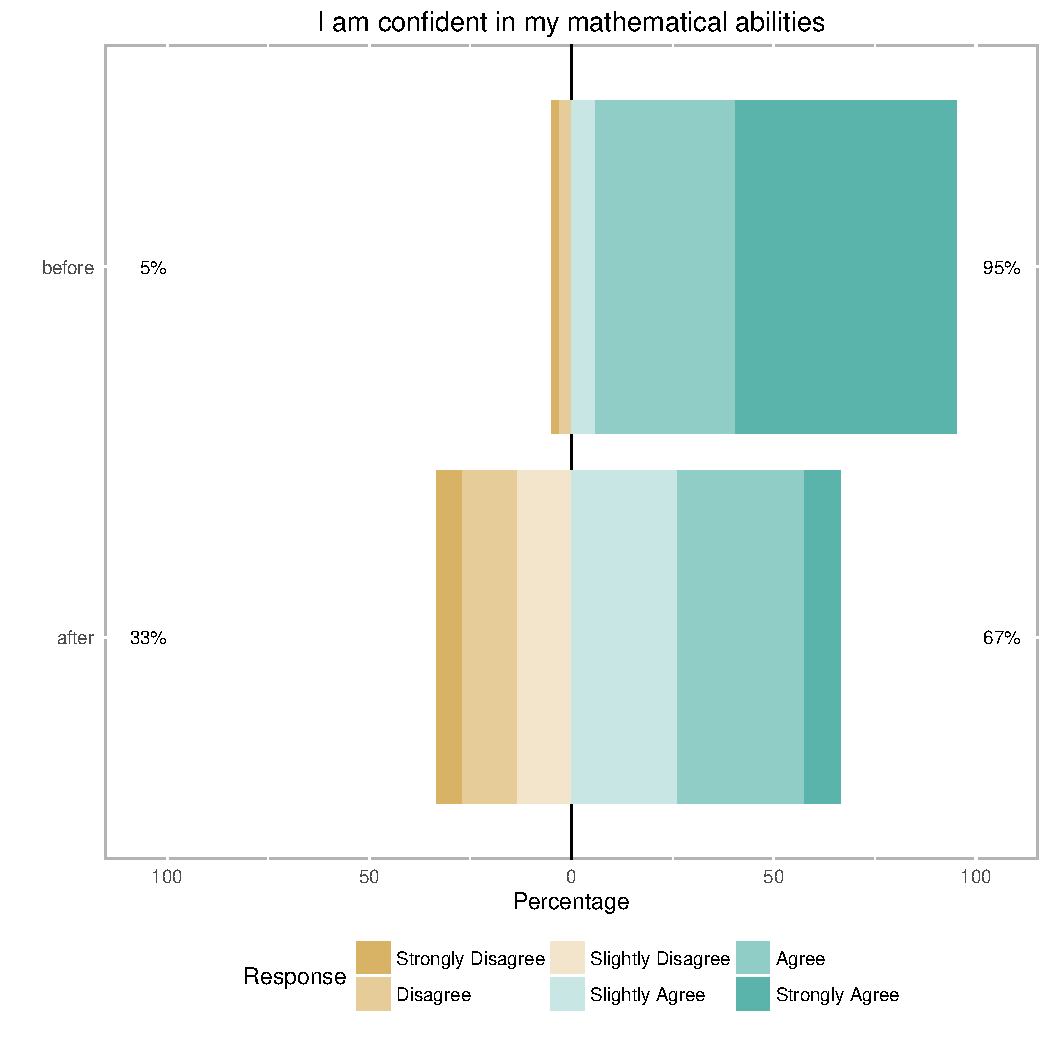
\includegraphics[height=\textheight]{graphs/confidence.pdf}
  \end{center}
\end{frame}

\clearbackgroundpicture
\begin{frame}
  \Large

  \frametitle{Research project}

  Ohio State's math department \\
  \quad studied various interventions \\
  \quad to improve outcomes in Calculus 1.

  \vfill

  Some sections use an \\
  \quad open-source Ximera-based text, \\
  while other sections \\
  \quad use a commercial text. \\

  \vfill

  Structured as a non-inferiority study.

\end{frame}

\begin{frame}
  \begin{center}
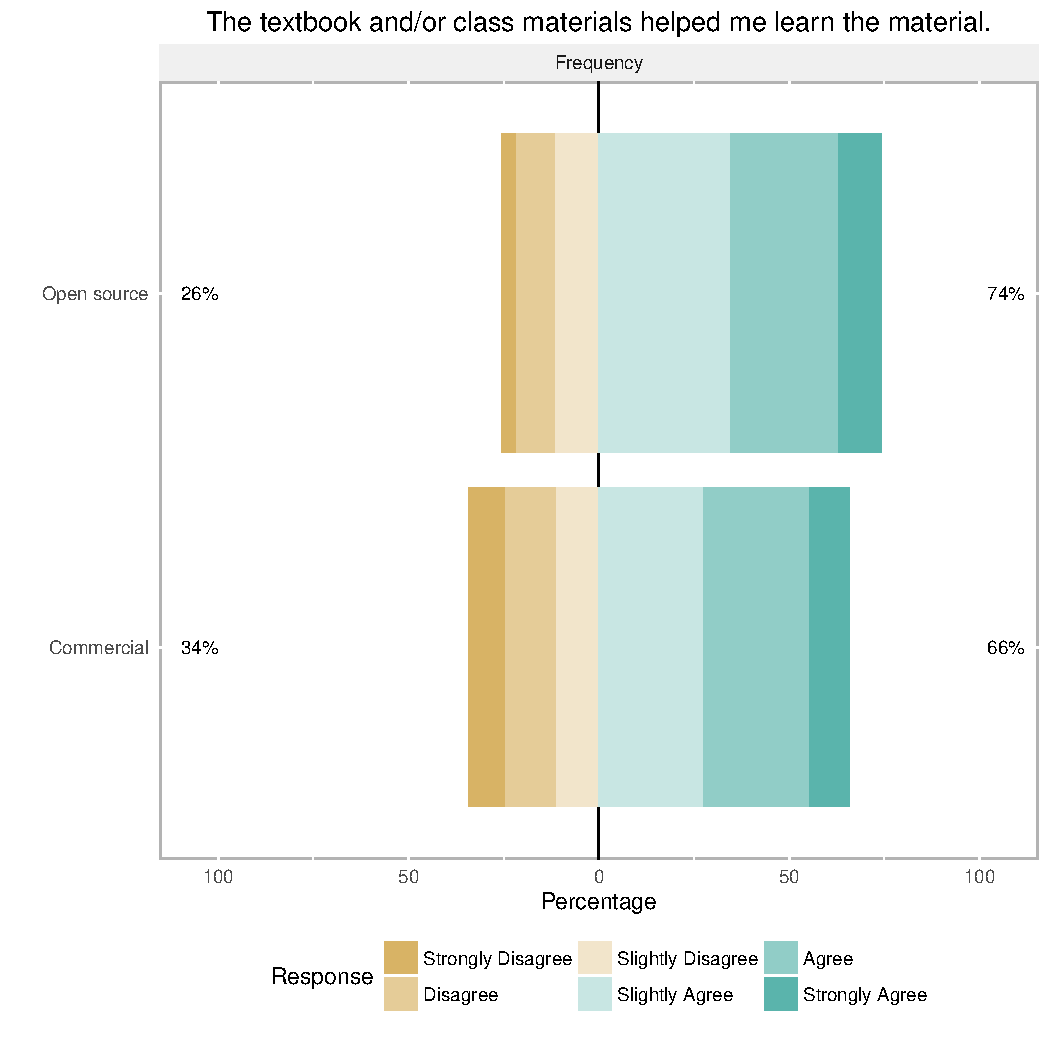
\includegraphics[height=\textheight]{graphs/textbook-helped-me.pdf}
  \end{center}
\end{frame}

\begin{frame}
  \begin{center}
    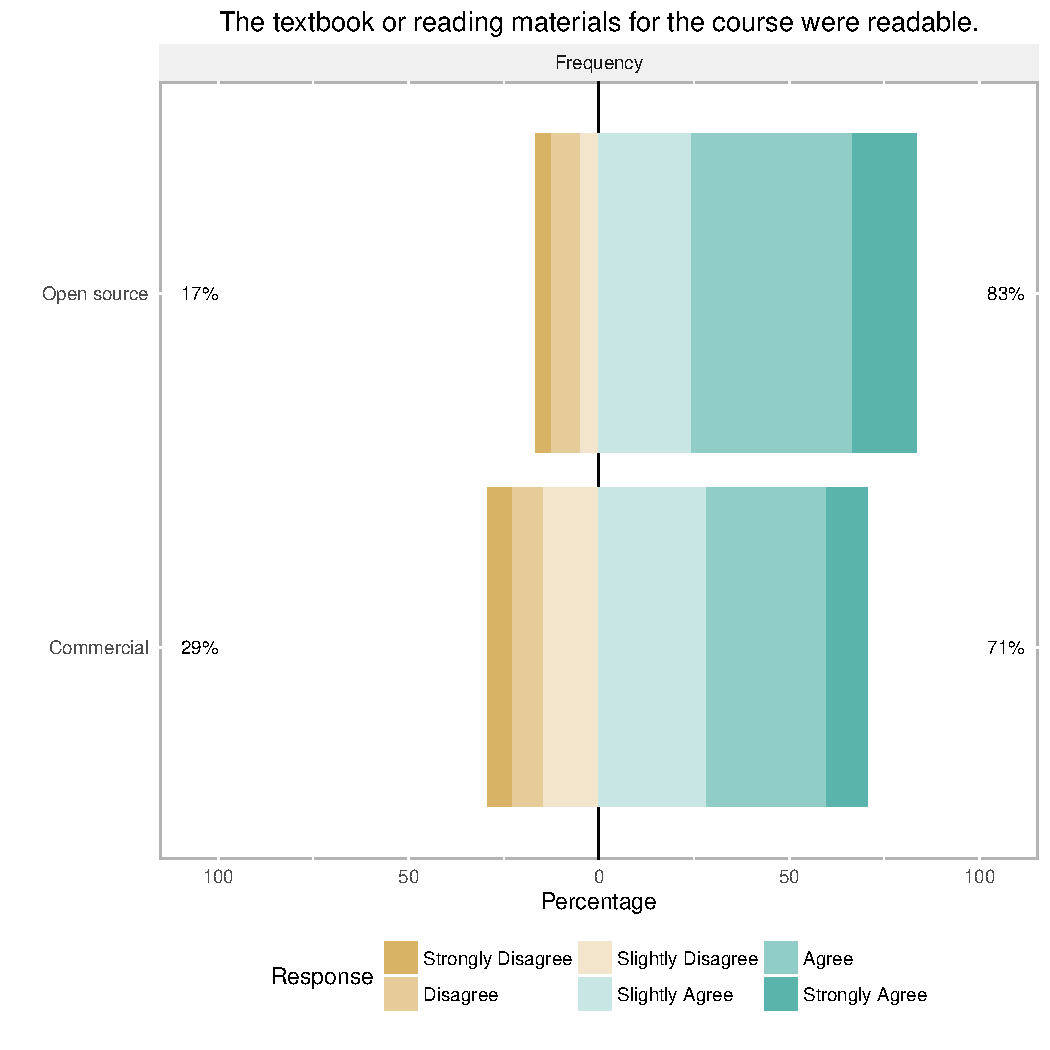
\includegraphics[height=\textheight]{graphs/textbook-readable.pdf}
  \end{center}
\end{frame}

\begin{frame}
  \frametitle{Weak affective improvements}

  Students in the open-source section were \\
  \quad more likely to express post-course \\
  \quad the same level or a stronger level of agreement with \\
  \quad the confidence item as pre-course \\
  \quad\quad\textcolor{gray}{\(OR =  1.42\), 95\% CI \([ 0.98 , 2.06 ]\),  \(p\approx 0.071\).}

  \vfill

  Students in the open-source section were \\
  \quad more likely to express post-course \\
  \quad the same level or a stronger level of agreement with \\
  \quad the enjoyment item as pre-course \\
  \quad\quad\textcolor{gray}{\(OR =  1.43\), 95\% CI \([ 0.98 , 2.1 ]\),  \(p\approx 0.072\).}
\end{frame}

\clearbackgroundpicture
%%%%%%%%%%%%%%%%%%%%%%%%%%%%%%%%%%%%%%%%%%%%%%%%%%%%%%%%%%%%%%%%
\begin{frame}[nofills]

  \vfill

  \scaletowidth{\textwidth}{\textbf{Thank You}}

  \vfill
  \begin{center}
    \begin{tabular}{rl}
      \textcolor{gray}{Email} & \texttt{ximera@math.osu.edu} \\
      \textcolor{gray}{Website} & \texttt{https://ximera.osu.edu/}
    \end{tabular}
  \end{center}
  \vfill
  \vfill
  \vfill
  
\includegraphics[width=1in]{cc-logo.pdf}\hfill\footnotesize\scalebox{0.75}{\textcolor{ccgray}{Licensed for reuse under a Creative Commons BY-NC-SA License}}
  \null
  % \vspace{12pt}
  \null
\end{frame}

\end{document}


%%%%%%%%%%%%%%%%%%%%%%%%%%%%%%%%%%%%%%%%%%%%%%%%%%%%%%%%%%%%%%%%
%%%%%%%%%%%%%%%%%%%%%%%%%%%%%%%%%%%%%%%%%%%%%%%%%%%%%%%%%%%%%%%%
%%%%%%%%%%%%%%%%%%%%%%%%%%%%%%%%%%%%%%%%%%%%%%%%%%%%%%%%%%%%%%%%



\begin{frame}
  \begin{center}
    \includegraphics[height=\textheight]{graphs/calculus-two.pdf}
  \end{center}
\end{frame}

\begin{frame}\Large
  \frametitle{Goal}

  Transform calculus so students \\
  \quad learn more math, \textcolor{gray}{and} \\
  \quad don't leave STEM.

\end{frame}

%%%%%%%%%%%%%%%%%%%%%%%%%%%%%%%%%%%%%%%%%%%%%%%%%%%%%%%%%%%%%%%%
\setbackgroundpictureblack{ximera/ximera.png}
\begin{frame}
\end{frame}

\setdarkbackgroundpictureblack{ximera/ximera.png}
\begin{frame}
  \vfill

  \color{white}
  \scaletowidth{\textwidth}{\texttt{https://ximera.osu.edu/}}

  \vfill
\end{frame}


\clearbackgroundpicture
\begin{frame}
The \textit{``users''} include \\
\begin{itemize}
\item Students enrolled in the course
\item Learners from the whole world
\item Instructors for credit
\item Authors of math content
\item Interactive widget authors
\item Other mathematicians looking for ideas on how to teach their own course
\item Education researchers
\item Web crawlers
\end{itemize}
\end{frame}

\clearbackgroundpicture
\encouragement{Why online homework?}

\begin{frame}[nofills]
  \frametitle{American Math Society Survey (2009)}

  \Large
  \vfill

  Among top eighty \\
  \quad Ph.D. granting math departments, \\
  \quad \textbf{67\%} use an online homework system.

  \vfill

  \uncover<2->{Most departments \\
    \quad who are using a homework system \\
    \quad are using a commercial system.}
  
  \vfill
  \scriptsize\url{http://www.ams.org/profession/leaders/WATSreport.pdf}
\end{frame}


\encouragement{Why textbooks?}

\begin{frame}
  \begin{center}
    \includegraphics[height=\textheight]{ximera/cover.pdf}
  \end{center}
\end{frame}

\clearbackgroundpicture
\begin{frame}
  \frametitle{Virginia Tech Study (2014)}
  \only<2>{\color{gray!50!white}} We analyzed the behavior of CS
  students when using the OpenDSA eTextbook system. We found that a
  \only<2>{\color{black}}majority of students skip directly to the
  exercises without reading the text, which indicates that the
  existing text is not engaging
  enough\only<2>{\color{gray!50!white}}\ or is too overwhelming for
  students. It is also possible that since most students waited until
  the due date to do the homework, \only<2>{\color{black}}reading the
  text was thought to ``slow them down'' so that they might not be
  able to submit the homework on time.
\end{frame}


\encouragement{\parbox{\widthof{Adoption of textbook}}{Adoption of textbook \\ \null\quad is adoption \\ of homework system.}}


%%%%%%%%%%%%%%%%%%%%%%%%%%%%%%%%%%%%%%%%%%%%%%%%%%%%%%%%%%%%%%%%

\begin{frame}
  \frametitle{Interactive Textbooks}
  \Large

  NSF DUE--1245433: \\
  \quad to create a platform for \\
  \quad\quad ``Interactive Textbooks.'' \pause\\
  \quad We call the platform ``Ximera.''

\end{frame}

\encouragement{Open Source FTW}

\begin{frame}
  \frametitle{YA Dystopian Novel}
  \Large

  \pause

   Instructors tell students \\
   \quad to pay the publisher \\
   \quad to receive homework points \\
   \quad to earn a course grade.

   \pause
   \vfill

   This outsources a core competency \\
   \quad of the University.

   \vfill

\end{frame}

\setbackgroundpictureblack{nature-license.png}
\begin{frame}
\end{frame}

\setdarkbackgroundpictureblack{nature-license.png}
\begin{frame}[nofills]
  \large
  \vfill
  \color{white}

  ``You may not sell, trade or otherwise transfer a Nature Education account to another party.''

  \vfill

  ``When you display \ldots material on \ldots the Site, it is provided \ldots under a license that is revocable.''

  \vfill

\end{frame}

\clearbackgroundpicture
\begin{frame}
  \huge

  \frametitle{YA Dystopian Novel}
  
  Don't lend your books.

  \vfill

  Don't expect to look \\
  \quad at ``your'' textbooks \\
  \quad in the future.

  \vfill

\end{frame}

\begin{frame}
  \frametitle{YA Dystopian Novel}
  
  The ``textbook filled with marginalia of an expert'' \\
  \quad is a conceit that appears in the Harry Potter
  series.
  
  \vfill
  \pause
  
  The technology we build \\
  \quad establishes the boundaries of the future world.

  \vfill
  \pause

  Does your homework system make it easier\ldots \\
  \quad for students to work together? \\
  \quad for students to have good conversations about math \\
  \quad\quad with each other \\
  \quad\quad\quad and with experts?
  
  \vfill
\end{frame}

\encouragement{Pedagogy not price}



%%%%%%%%%%%%%%%%%%%%%%%%%%%%%%%%%%%%%%%%%%%%%%%%%%%%%%%%%%%%%%%%
\begin{frame}
  \textbf{Question:} \\
  \quad Why is ``search'' for instructional materials so bad?

  \vfill\vfill\pause

  A lack of metadata?

  \vfill\pause

  A lack of great content?

  \vfill\pause

  Or because content is locked behind various walls?

  \vfill\vfill
\end{frame}

\encouragement{The Open Web}

\settallbackgroundpictureblack{wikipedia.png}
\begin{frame}
\end{frame}

\clearbackgroundpicture
\begin{frame}
  Wikipedia is good because it is\ldots
  \begin{itemize}
  \item editable by me
  \item bookmarkable and shareable with URLs
  \item stored in plain text
  \item licensed for reuse
  \item curated by experts
  \item works on my phone
  \item links to other content
  \end{itemize}

  \vfill\pause

  Wikipedia isn't so good because\ldots\pause \\
  \quad\textbf{WHERE ARE THE EXERCISES?!}
  
\end{frame}

% BADBAD: picture of ximeragrat

\begin{frame}[nofills]
  \frametitle{What is Ximera?}

  \vspace{-0.35in}\includegraphics[width=\textwidth]{ximera/infographic.pdf}
\end{frame}
%%%%%%%%%%%%%%%%%%%%%%%%%%%%%%%%%%%%%%%%%%%%%%%%%%%%%%%%%%%%%%%%
\setbackgroundpictureblack{ximera/ximera-calculus.png}
\begin{frame}
\end{frame}

\setdarkbackgroundpictureblack{ximera/ximera-calculus.png}
\begin{frame}[nofills]
\vfill\color{white}
\begin{center}
\Huge\textsf{\textbf{\scaletowidth{0.75\textwidth}{\stacksame{Calculus}{content}}}}
\end{center}
\vfill
\end{frame}


\setdarkbackgroundpictureblack{ximera/ximera-page.png}
\begin{frame}[nofills]
\vfill\color{white}
\begin{center}
\Huge\textsf{\textbf{\scaletowidth{0.75\textwidth}{\stacksame{on the web}{or on paper}}}}
\end{center}
\vfill
\end{frame}

%%%%%%%%%%%%%%%%%%%%%%%%%%%%%%%%%%%%%%%%%%%%%%%%%%%%%%%%%%%%%%%%
\setbackgroundpictureblack{ximera/ximera-multiple-choice.png}
\begin{frame}
\end{frame}

\setdarkbackgroundpictureblack{ximera/ximera-multiple-choice.png}
\begin{frame}[nofills]
\vfill\color{white}
\begin{center}
\Huge\textsf{\textbf{\scaletowidth{0.75\textwidth}{\stacksame{multiple}{choice}}}}
\end{center}
\vfill
\end{frame}

%%%%%%%%%%%%%%%%%%%%%%%%%%%%%%%%%%%%%%%%%%%%%%%%%%%%%%%%%%%%%%%%
% Mobile
\clearbackgroundpicture
\usebackgroundtemplate{%
\begin{tikzpicture}[overlay,remember picture]%
\draw[fill=black] (current page.north west) rectangle (current page.south east);%
\node[minimum width=\paperwidth,minimum height=\paperheight,yshift=1.5mm] [anchor=north west] (mynode) {};%
\draw[fill=black,opacity=0.75] (current page.north west) rectangle (current page.south east);%
\end{tikzpicture}%
}
\begin{frame}
  \blackbackground
  \begin{columns}
    \begin{column}{0.5\textwidth}
      \includegraphics[width=\textwidth]{ximera/mobile.jpg}
    \end{column}
    \begin{column}{0.5\textwidth}
      \vfill
      \color{white}
      \scaletowidth{\textwidth}{Mobile}
      \vfill
    \end{column}
  \end{columns}
\end{frame}

%%%%%%%%%%%%%%%%%%%%%%%%%%%%%%%%%%%%%%%%%%%%%%%%%%%%%%%%%%%%%%%%
\setbackgroundpictureblack{ximera/ximera-math-answer.png}
\begin{frame}
\end{frame}

\setdarkbackgroundpictureblack{ximera/ximera-math-answer.png}
\begin{frame}[nofills]
\vfill\color{white}
\begin{center}
\Huge\textsf{\textbf{\scaletowidth{0.75\textwidth}{\stacksame{mathematical}{expressions}}}}
\end{center}
\vfill
\end{frame}


\clearbackgroundpicture
\begin{frame}\Large
  \frametitle{Metrics}
  
  \begin{description}
  \item[Conceptual] pre- and post-tests;
  \item[Surveys] from the \textit{Characteristics of Successful Programs in College Calculus} (CSPCC) study; \textcolor{gray}{and}
  \item[Common exams] across all sections.
  \end{description}
\end{frame}

\newcommand{\intervention}[1]{\scshape{#1}}
\newcommand{\XIMERA}{X\hsc{imera}}
\newcommand{\ACTIVE}{A\hsc{ctive}}
\newcommand{\FLIPPED}{F\hsc{lipped}}
\newcommand{\BIGCLASS}{H\hsc{uge}}
\newcommand{\SMALLCLASS}{E\hsc{psilon}}
\newcommand{\TRADITIONAL}{T\hsc{raditional}}

\begin{frame}
  \frametitle{Five Interventions and Control}

  \begin{description}[\TRADITIONAL]
    \item[\TRADITIONAL] 180-student lecture and 32-student recitations
    \item[\XIMERA] an open-source text and homework system
    \item[\ACTIVE] with peer instruction and clickers
    \item[\FLIPPED] meeting twice/week and online
    \item[Class size] both large (\makebox[0in][l]{\raisebox{-14pt}{\uncover<2->{\textcolor{gray}{384 students}}}}\BIGCLASS) and small (\makebox[0in][l]{\raisebox{-14pt}{\uncover<2->{\textcolor{gray}{32 students}}}}\SMALLCLASS)
  \end{description}

\end{frame}

\begin{frame}
  \begin{center}
    \includegraphics[height=\textheight]{graphs/contributed-to-discussion.pdf}
  \end{center}
\end{frame}


\begin{frame}
  \frametitle{A day in \FLIPPED}

  On Monday, Wednesday, and Friday, \\
  \quad students complete online lessons\\
  \quad\quad instead of attending lecture.

  \vfill

  On Tuesdays and Thursdays, \\
  \quad students attend recitation \\
  \quad\quad either in person or \\
  \quad\quad synchronously through the web.

  \vfill

  Recitations are centered around active learning \\
  \quad with students working on problems in groups.
\end{frame}


\begin{frame}
  \begin{center}
    \includegraphics[height=\textheight]{graphs/flipped-versus-traditional.pdf}
  \end{center}
\end{frame}

\begin{frame}
  \begin{center}
    \includegraphics[height=\textheight]{graphs/academic-level.pdf}
  \end{center}
\end{frame}

\begin{frame}
  \frametitle{A day in \ACTIVE}

  Class consists of a short (10--15 minutes) lecture, \\
  \quad a question presented online, \\
  \quad peer instruction and discussion of responses, \\
  \quad a whole class discussion, \\
  \quad a summary of the correct response, \\
  and repeat.

  \vfill

  Recitations consist of students \\
  \quad working in small groups on worksheets, \\
  \quad followed by whole class discussions.
\end{frame}

\begin{frame}
  \begin{center}
    \includegraphics[height=\textheight]{graphs/whole-discussion-frequency-summary.pdf}
  \end{center}
\end{frame}

%\begin{frame}
%  \begin{center}
%    \includegraphics[height=\textheight]{graphs/student-explanation-frequency.pdf}
%  \end{center}
%\end{frame}

\begin{frame}
  \begin{center}
    \includegraphics[height=\textheight]{graphs/student-explanation-frequency-summary.pdf}
  \end{center}
\end{frame}

\begin{frame}
  \begin{center}
    \includegraphics[height=\textheight]{graphs/exam-scores.pdf}
  \end{center}
\end{frame}

\begin{frame}
  \begin{center}
    \includegraphics[height=\textheight]{graphs/exam-scores-year.pdf}
  \end{center}
\end{frame}


\encouragement{\textit{Cui bono?}}

\clearbackgroundpicture
\begin{frame}
  \begin{center}
    \includegraphics[height=\textheight]{nwna/all-understand.pdf}
  \end{center}
\end{frame}

\begin{frame}
  \begin{center}
    \includegraphics[height=\textheight]{nwna/nwna-understand.pdf}
  \end{center}
\end{frame}

\begin{frame}
  \begin{center}
    \includegraphics[height=\textheight]{nwna/all-interest.pdf}
  \end{center}
\end{frame}

\begin{frame}
  \begin{center}
    \includegraphics[height=\textheight]{nwna/nwna-interest.pdf}
  \end{center}
\end{frame}

\begin{frame}
  \begin{center}
    \includegraphics[height=\textheight]{graphs/predicted-actual-traditional.pdf}
  \end{center}
\end{frame}

\begin{frame}
  \begin{center}
    \includegraphics[height=\textheight]{graphs/predicted-actual-ximera.pdf}
  \end{center}
\end{frame}



%\begin{frame}
%  \begin{center}
%    \includegraphics[height=\textheight]{graphs/use-technology.pdf}
%  \end{center}
%\end{frame}

%\begin{frame}
%  \begin{center}
%    \includegraphics[height=\textheight]{graphs/group-work-frequency.pdf}
%  \end{center}
%\end{frame}

%\begin{frame}
%  \begin{center}
%    \includegraphics[height=\textheight]{graphs/group-work-frequency-summary.pdf}
%  \end{center}
%\end{frame}

%\begin{frame}\large
%  \frametitle{Claim}

%  There are real differences \\
%  \quad between \TRADITIONAL\ and \\
%  \quad the other sections.
%\end{frame}


%%%%%%%%%%%%%%%%%%%%%%%%%%%%%%%%%%%%%%%%%%%%%%%%%%%%%%%%%%%%%%%%
%\encouragement{\ACTIVE}



%\begin{frame}
%  \begin{center}
%    \includegraphics[height=\textheight]{graphs/confidence-change.pdf}
%  \end{center}
%\end{frame}

%%%%%%%%%%%%%%%%%%%%%%%%%%%%%%%%%%%%%%%%%%%%%%%%%%%%%%%%%%%%%%%%







%\begin{frame}
%  \begin{center}
%    \includegraphics[height=\textheight]{graphs/calculus-two-begin.pdf}
%  \end{center}
%\end{frame}

%\begin{frame}
%  \begin{center}
%    \includegraphics[height=\textheight]{graphs/calculus-two-ending.pdf}
%  \end{center}
%\end{frame}





% BADBAD include tables and graphs

%%%%%%%%%%%%%%%%%%%%%%%%%%%%%%%%%%%%%%%%%%%%%%%%%%%%%%%%%%%%%%%%
\encouragement{GitHub}

\settallbackgroundpicturewhite{github/mooculus.png}
\begin{frame}
\end{frame}

\settalldarkbackgroundpicturewhite{github/mooculus.png}
\begin{frame}[nofills]
\vfill
\begin{center}
\Huge\textsf{\textbf{\scaletowidth{0.75\textwidth}{\stacksame{Version}{\stacksame{controlled}{repository}}}}}
\end{center}
\pause
\vfill
\begin{center}
\large\texttt{https://github.com/mooculus/calculus1}
\end{center}
\vfill
\vfill
\end{frame}

\settallbackgroundpicturewhite{github/commits.png}
\begin{frame}
\end{frame}

\settalldarkbackgroundpicturewhite{github/commits.png}
\begin{frame}[nofills]
\vfill
\begin{center}
\Huge\textsf{\textbf{\scaletowidth{0.75\textwidth}{\stacksame{History of}{changes}}}}
\end{center}
\vfill
\end{frame}

%%%%%%%%%%%%%%%%%%%%%%%%%%%%%%%%%%%%%%%%%%%%%%%%%%%%%%%%%%%%%%%%

\settallbackgroundpicturewhite{github/textbook-sample.png}
\begin{frame}
\end{frame}

\settalldarkbackgroundpicturewhite{github/textbook-sample.png}
\begin{frame}[nofills]
\vfill
\begin{center}
\Huge\textsf{\textbf{\scaletowidth{0.75\textwidth}{\stacksame{Anyone}{can edit}}}}
\end{center}
\vfill
\end{frame}

%%%%%%%%%%%%%%%%%%%%%%%%%%%%%%%%%%%%%%%%%%%%%%%%%%%%%%%%%%%%%%%%
\settallbackgroundpicturewhite{github/contribution.png}
\begin{frame}[label=students-edit-1]
\end{frame}

\settalldarkbackgroundpicturewhite{github/contribution.png}
\begin{frame}[nofills]
\vfill
\begin{center}
\Huge\textsf{\textbf{\scaletowidth{0.75\textwidth}{\stacksame{Students}{make edits}}}}
\end{center}
\vfill
\end{frame}

\clearbackgroundpicture
\begin{frame}
  \frametitle{Design Principles}

  \begin{itemize}
  \item editable by students
  \item curated by the instructor
  \item math content authored in \LaTeX \\
    \quad and interactive content in JavaScript 
  \item licensed for reuse
  \item works on phones
  \item content is versioned via \texttt{git}
  \item event stream logged with xAPI
  \end{itemize}

\end{frame}

\encouragement{The Future}

\setbackgroundpictureblack{ipfs.png}
\begin{frame}
\end{frame}

\setbackgroundpictureblack{ethereum.jpg}
\begin{frame}
\end{frame}

\settallbackgroundpictureblack{peer-review.png}
\begin{frame}
\end{frame}

\clearbackgroundpicture
\begin{frame}
  \begin{center}
    \includegraphics[height=\textheight]{graphs/normalized-gains.pdf}
  \end{center}
\end{frame}

\begin{frame}
  \frametitle{P11}

  The graph of the position of an object with respect to time is given
  by a straight line with a positive slope.

  What can we say about the acceleration of the object?
  \begin{itemize}
    \item{It is positive.}
    \item{It is negative.}
    \item{It is zero.}
    \item{The acceleration changes from negative to positive.}
    \item{We cannot say anything about the sign of the acceleration.}
  \end{itemize}

\end{frame}

\begin{frame}
  \begin{center}
    \includegraphics[height=\textheight]{graphs/p11.pdf}
  \end{center}
\end{frame}

\begin{frame}
  \frametitle{P13}

  Four equally spaced numbers are shown below on a number line.
  \begin{center}
    \begin{tikzpicture}[x=0.19\textwidth]
      \draw[-{>[scale=1.75]}] (-0.05\textwidth,0) -- (0.8\textwidth,0);
      \foreach \x in {0,...,4} {%
        \draw (\x,-.1) -- (\x,.1);
        \node[anchor=north,yshift=-2pt] at (\x,0) {$\x$};
      }
      \draw (0.5,0) node [circle,fill,inner sep=1pt,label=above:$x$](e){};
      \draw (1.5,0) node [circle,fill,inner sep=1pt,label=above:$y$](e){};
      \draw (2.5,0) node [circle,fill,inner sep=1pt,label=above:$z$](e){};
      \draw (3.5,0) node [circle,fill,inner sep=1pt,label=above:$w$](e){};
    \end{tikzpicture}
  \end{center}

  Let $f(t) = \ln t$ and consider $f(x)$ and $f(y)$ and $f(z)$ and
  $f(w)$.  Among the pairs listed below, which pair of numbers is
  farthest apart?
  \begin{itemize}
    \item{The pair $f(x)$ and $f(y)$.}
    \item{The pair $f(y)$ and $f(z)$.}
    \item{The pair $f(z)$ and $f(w)$.}
    \item{These pairs are all equally far apart.}
  \end{itemize}

\end{frame}

\begin{frame}
  \begin{center}
    \includegraphics[height=\textheight]{graphs/p13.pdf}
  \end{center}
\end{frame}

\begin{frame}
  \begin{center}
    \includegraphics[height=\textheight]{graphs/cka-problem-p13-and-p11.pdf}
  \end{center}
\end{frame}

\begin{frame}
  \frametitle{Themes of the Future}
  
  \begin{itemize}
  \item Decentralized content distributed through IPFS
  \item Grading free response through clustering
  \item Mobile and VR
  \item Big data and analytics
  \item No single textbook; multiple sites
  \item Iterative loops for course designers and for students
  \end{itemize}

\end{frame}

\begin{frame}
  \frametitle{E-Commerce as a model}

  The most personalized part of the internet is advertising.

  If you want learning to be personalized, \\
  \quad make it work like ads.

  \vfill\pause

  \begin{itemize}
  \item An analytics backend to do A/B testing \\
    \quad (like git branches) 
  \item A common ``event stream'' for conversions \\
    \quad (like the xAPI and an LRS)
  \item An advertising network for sharing content \\ 
    \quad (like CuratedCourses)
  \end{itemize}

\end{frame}

\begin{frame}
  \frametitle{Worry about workflow}

  \large
  \begin{description}[Researchers]
  \item[Authors] write in a safe place.
  \item[Learners] access exercises without logging in.
  \item[Researchers] get event stream data.
  \end{description}
\end{frame}

 %%%%%%%%%%%%%%%%%%%%%%%%%%%%%%%%%%%%%%%%%%%%%%%%%%%%%%%%%%%%%%%%
 \clearbackgroundpicture
 \begin{frame}[label=thanks,nofills]
   \vfill
   \begin{center}
   \Huge
    \scalebox{1.5}{\textbf{Thank You}}
   \end{center}
   \vfill
   \vfill
   
\includegraphics[width=1in]{images/cc-logo.pdf}\hfill\footnotesize\scalebox{0.75}{\textcolor{ccgray}{Licensed for reuse under a Creative Commons BY-NC-SA License}}
   \null
   %\vspace{12pt}
   \null
 \end{frame}



%Sad XML Truth No. 3: Interoperability isn�t an engineering issue,
%it�s a business issue.  Creating the Web -- HTTP plus HTML -- was
%probably the last instance where standards of global importance were
%designed and implemented without commercial interference. Standards
%have become too important as competitive tools to leave them where
%they belong, in the hands of engineers. Incompatibility doesn't exist
%because companies can't figure out how to cooperate with one
%another. It exists because they don�t want to cooperate with one another.

\end{document}
